%%%%%%%%%%%%%%%%%%%%%%%%%%%%%%%%%%%%%%%%%%%%%%%%%%%%%%%%%%%%%%%%%%%%%%
%Exemple de structuration de thèse utilisant le format Latex

\pagestyle{fancy}

\newgeometry{lmargin=20mm,tmargin=30mm,rmargin=20mm,bmargin=30mm,headsep=10mm,footskip=20mm,bindingoffset=10mm}
\usefont{T1}{cmr}{m}{n}

\frontmatter
\section*{Remerciements}
\lipsum[17-19]

\newpage

\tableofcontents
\addcontentsline{toc}{part}{Liste des figures}
\listoffigures
\addcontentsline{toc}{part}{Liste des tables}
\listoftables
%%%%%%%%%%%%%%%%%%%%%%%%%%%%%%%%%%%%%%%%%%%%%%%%%%%%%%%%%%%%%%%%%%%%%
\mainmatter

\part{Introduction}
\section{Un peu de contexte}

\subsection{Les acteurs}
\paragraph{}
Ces travaux sont menés conjointement par le \gls{lifo} et la société \gls{ennov}.
\gls{ennov} est un éditeur de logiciels spécialisé dans le domaine médical.
Ils proposent une suite logicielle pour la gestion de contenus ainsi que l’automatisation des processus métier et des processus réglementaires.
Cela permet aux sociétés des sciences de la vie de réduire les risques réglementaires et de faciliter le respect des normes internationales.
\gls{ennov} est certifié ISO9001: 2015 pour tous ses produits et activités.
Ils offrent une meilleure capacité de prise de décision, une automatisation des tâches répétitives et une visibilité accrue dans toute l'organisation.
\gls{ennov} est hautement évolutif, mais facilement implémenté, conçu pour une utilisation minimale de l'infrastructure informatique, des coûts ou des ressources.

\gls{ennov} est reconnu par \gls{gartner} comme un fournisseur pertinent pour le \gls{rim} / \gls{idmp} ainsi qu'un fournisseur mondial de technologies logicielles pour les sociétés des sciences de la vie.
La suite logicielle d'\gls{ennov} comprend des fonctions de gestion de processus et de contenu pour la gestion de la qualité, les affaires réglementaires, les études cliniques et la pharmacovigilance.

\gls{ennov} a pour objectif de concevoir des solutions logicielles interconnectées qui s'intègrent aux flux de travail.
L'ensemble de la suite logicielle est basée sur une \gls{ged} qui est chargée de la gestion du cycle de vie des documents.
Ces travaux vont permettre une meilleure utilisation des données disponibles afin d'obtenir des gains de productivité.

\paragraph{}
Le \gls{lifo} est un laboratoire de l'université d'Orléans et de l'\gls{insa} Centre-Val de Loire.
Les recherches qui sont menées au \gls{lifo} vont de l'algorithmique au traitement des langues naturelles, de l'apprentissage au parallélisme massif, de la vérification et la certification à la sécurité des systèmes, du Big Data aux systèmes embarqués.

Le \gls{lifo} est composé de cinq équipes :
\begin{description}
 \item[CA] Contraintes et Apprentissage
 \item[GAMoC] Graphes, Algorithmes et Modèles de Calcul
 \item[LMV] Logique, Modélisation et Vérification
 \item[Pamda] Parallélisme, Calcul distribué et Base de donnés
 \item[SDS] Sécurité des Données et des Systèmes
\end{description}

\section{Le projet}
L'extraction des informations contenues dans un texte, sa structuration, sa classification et son étude statistiques représente un challenge, mais aussi une grande plus-value concernant le domaine de la pharmacovigilance.
Ce dernier consiste à suivre les cas d'effet secondaire liée à différents médicaments.
Il est important de connaître l'historique de chaque patient ainsi que le déroulement précis des évènements pour déduire la cause des effets secondaires.
Ces informations sont recueillies par des centres d'appels qui ont pour mission de fournir un document standardisé auprès des autorités de santé.
Comme dit précédemment les informations contenues dans ce document, pourtant essentiel pour déduire les causes, ne sont pas accessibles par un traitement automatique.
Il est donc nécessaire de fournir manuellement toutes ces informations.
Cela représente une grande quantité de données et donc un temps de travail et un coût plus important sans oublier que c'est un processus à fort risque d'erreur.

La pharmacovigilance est donc l'emploi idéal de telle recherche, car il est important de pouvoir extraire cette information et de faciliter, par la suite, leur compréhension et leur analyse avec des requêtes plus évoluées permettant à l'avenir de concevoir un système-expert.
Ces travaux ont pour vocation d'être intégré à la suite \gls{ennov} que ce soit dans la \gls{ged} ou dans la partie logicielle traitant de la pharmacovigilance.

\paragraph{}
L'interrogation du contenu des documents implique que ces données soient facilement accessibles et de façon structurée, ce qui n'est pas le cas dans un document textuel.
Le projet se découpe donc en deux axes, dans un premier temps, il s'agit d'extraire l'information, la structurer et la stocker.
Dans un second temps, il faut proposer un formalisme d'interrogation basé sur le contexte permettant des analyses statistiques dans une base de données et permettre la traduction d'une requête en langage naturel vers ce formalisme.

\paragraph{}
Pour construire une base de connaissance cohérente et structurée, il faut commencer par extraire les données contenues dans les documents.
Ce processus se nomme : \gls{ie} (\cite{grishman_information_1997,cowie_information_2000}) et représente un axe de recherche du \gls{tal}.
Certains travaux portent déjà sur l'extraction d'information notamment dans un domaine médical \cite{polepalli_ramesh_automatically_2014}, cependant, ils ne permettent pas d'obtenir une structure cohérente pour ces données et il est donc peu envisageable de tenter d'y retrouver de l'information sans un traitement préalable.
N'existant pas de solution nous permettant d'obtenir le résultat souhaité, ceci constitue un des axes de recherche du projet.

Le second axe de recherche porte sur la formulation de requête statistique enrichie d'un contexte \cite{chabin_context-driven_2018}.
Le contexte est une suite de règles permettant de préciser la requête initiale.
Dans le cadre du projet, ces travaux rendront personnalisé les requêtes utilisateurs, car chacun se verra attribuer un contexte qui lui est propre.
Le contexte servira aussi pour l'extraction d'information.

\paragraph{}
Le projet est donc découpé en plusieurs parties regroupées sous différents modules.
La figure~\ref{fig:sch_projet} présente les cinq modules du projet ainsi que les différentes parties en précisant les travaux qui les lient.

\begin{figure}[htb]
    \centering
    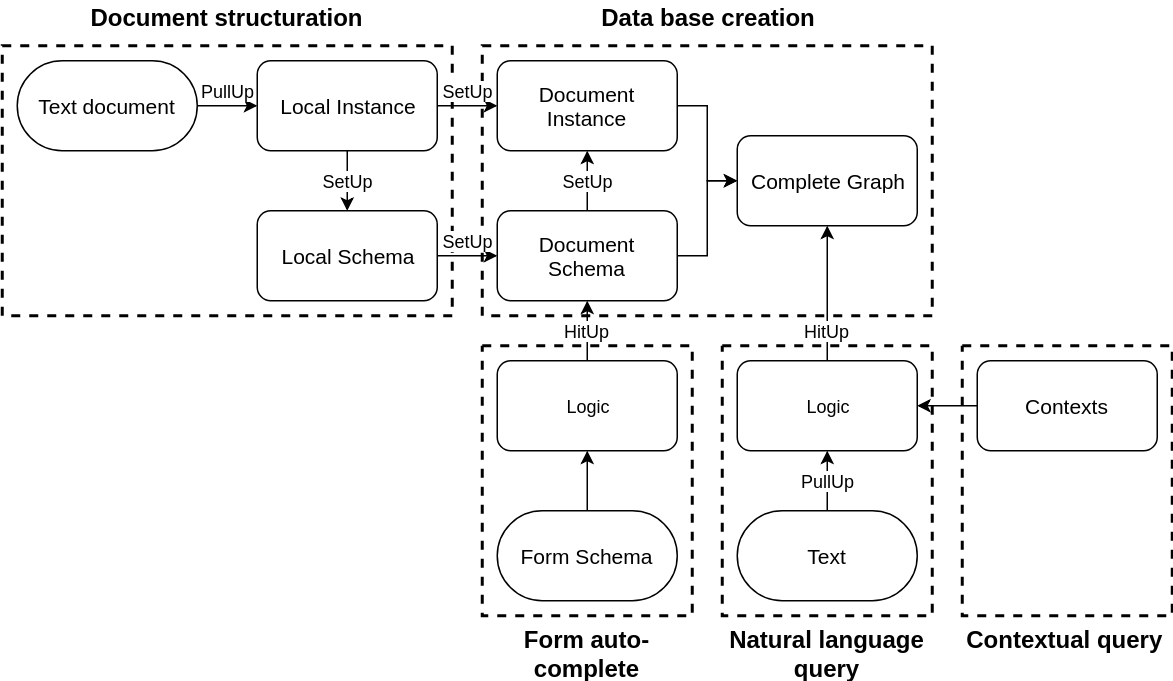
\includegraphics[width=\linewidth]{these/images/global_project.png}
    \caption{Schéma du projet}
    \label{fig:sch_projet}
\end{figure}

\paragraph{\gls{pullup}} est la partie s'occupant de l'extraction d'information.
Elle a pour objectif d'extraire les connaissances contenues dans un texte formulé en langage naturel sous forme de faits logique pouvant être utilisés pour construire notre base de données par la suite.

\paragraph{\gls{setup}} est un ensemble de travaux visant à construire dynamiquement une base de données cohérente par l'intermédiaire de grammaire de graphe \cite{chabin_using_2019}.
Ces travaux sont réalisés conjointement avec l'équipe SDS du \gls{lifo}.
Ils devraient permettre de s'assurer que la base reste cohérente sachant que l'on ne connaît pas la structure des données en entrée (car elles sont extraites depuis différents documents) et qu'on ne connaît pas le schéma de notre base (le schéma est propre aux documents présents dans la \gls{ged} et donc propre à chaque client).
Bien que le processus puisse être réalisé manuellement, cette partie du projet vise donc à automatiser la construction de la base spécifique permettant de formuler des requêtes plus adaptées aux données qu'elle contient.

\paragraph{\gls{hitup}} est une extension du formalisme présenté par \cite{chabin_context-driven_2018}.
Il vise à fournir un langage de requête permettant d'effectuer des requêtes statistiques tout en ajoutant, via des réécritures, un contexte à la requête.
Ce dernier peut être composé de contraintes d'intégrité ou de règles d'inférence utilisées pour spécifier la requête.

\section{Exemple}
\begin{quote}
    Un patient de 78 ans suivi pour cancer prostatique avec métastases ganglionnaires ayant déjà subi une résection endoscopique prostatique avec pulpectomie a été admis en urgence pour insuffisance rénale aiguë obstructive à 330 mmol/l de créatinine avec fièvre et urétérohydronéphrose bilatérale à l'échographie.
\end{quote}

\begin{align}
    CasClinique(\textit{c-2-3})  & exam(p_1, e_1, et_1, \textit{01-01-01}) \\
    hasPatient(\textit{c-2-3}, p1) & paramClinique(e_1, creatine, \textit{330mmol/L}) \\
    Patient(p_1, 78, H)  & reveal(e_1, \textit{insuffisance rénale}) \\
    hasPatho(p_1, cancer)  & exam(p_1, e_2, et_2, \textit{01-01-01}) \\
    concernsAnat(cancer, prostate) & paramClinique(e_2, temperature, t_1) \\
    Anatomy(prostate)  & reveal(e_2, fievre)  & exam(p_1, e_3, \textit{echographie}, \textit{01-01-01}) \\
    leadTo(cancer, \textit{métastases ganglionnaires})  & paramClinique(e_3, param_1, res_1) \\
    getTreatment(\textit{résection endoscopique}, prostate) & reveal(e_3, \textit{urétérohydronéphrose bilatérale}) \\
    forPatho(\textit{résection endoscopique}, cancer)
\end{align}

\begin{figure}
    \small
    \centering
    \begin{adjustbox}{varwidth=\linewidth,max height=\textheight}
        \begin{tikzpicture}[shorten >=2pt,thick,-Latex,node distance=3cm and 5cm,on grid]
            \node[labeled node] (patient) {Patient \nodepart{two} name: \emph{$p_1$}\\sex: \emph{H}\\age: \emph{78}};
            \node[labeled node, below=of patient] (exam1) {Exam \nodepart{two} name: \emph{constantes}};
            \node[labeled node, below=of exam1] (param1) {ParamClinique \nodepart{two} name: \emph{créatinine}\\value: \emph{330 mmol/l}};
            \node[labeled node, below=of param1] (sosy1) {SOSY \nodepart{two} name: \emph{insuffisance}\\~~~~~~~~~~\emph{rénale}};
            \node[labeled node, right=of exam1] (exam2) {Exam \nodepart{two} name: \emph{échographie}};
            \node[labeled node, below=of exam2] (param2) {ParamClinique \nodepart{two} name: \emph{unknown}\\ value: \emph{unknown}};
            \node[labeled node, below=of param2] (sosy2) {SOSY \nodepart{two} name: \emph{urétérohydronéphrose}\\~~~~~~~~~~\emph{bilatérale}};
            \node[labeled node, left=of param1] (param3) {ParamClinique \nodepart{two} name: \emph{temperature}\\ value: \emph{unknown}};
            \node[labeled node, below=of param3] (sosy3) {SOSY \nodepart{two} name: \emph{fièvre}};
            \node[labeled node, above=of param3] (cas) {CasClinique \nodepart{two} doc: \emph{c-2-3}};
            \node[labeled node, above=of cas] (testicule) {Anatomie \nodepart{two} name: \emph{testicule}};
            \node[labeled node, above=of patient] (traitement) {Traitement};
            \node[labeled node, above=of traitement] (traitmentType) {TraitmentType \nodepart{two} name: \emph{résection}\\~~~~~~~~~~\emph{endoscopique}};
            \node[labeled node, above=of testicule] (traitement2) {Traitement};
            \node[labeled node, above=of traitement2] (traitmentType2) {TraitmentType \nodepart{two} name: \emph{pulpectomie}};
            \node[labeled node, above=of exam2] (metastase) {Symptom \nodepart{two} name: \emph{métastases}\\~~~~~~~~~~\emph{ganglionnaires}};
            \node[labeled node, above=of metastase] (cancer) {Pathologie \nodepart{two} name: \emph{cancer}};
            \node[labeled node, above=of cancer] (prostate) {Anatomie \nodepart{two} name: \emph{prostate}};

            \path
            (cas) edge node[labeled edge, anchor=center] {hasPatient} (patient)
            (patient) edge node[labeled edge, anchor=center] {hasPatho} (cancer)
            (patient) edge node[labeled edge, anchor=center] {getTreatment} (traitement)
            (cancer) edge node[labeled edge, anchor=center] {concernsAnat} (prostate)
            (patient) edge node[labeled edge, anchor=center] {getTreatment} (traitement2)
            (cancer) edge node[labeled edge, anchor=center] {leadTo} (metastase)
            (traitement) edge node[labeled edge, anchor=center] {forPatho} (cancer)
            (traitement) edge node[labeled edge, anchor=center] {concernsAnat} (prostate)
            (traitement) edge node[labeled edge, anchor=center] {hasType} (traitmentType)
            (traitement2) edge node[labeled edge, anchor=center] {concernsAnat} (testicule)
            (traitement2) edge node[labeled edge, anchor=center] {hasType} (traitmentType2)
            (patient) edge node[labeled edge, anchor=center] {passExam} (exam1)
            (exam1) edge node[labeled edge, anchor=center] {reveal} (param1)
            (param1) edge node[labeled edge, anchor=center] {show} (sosy1)
            (patient) edge node[labeled edge, anchor=center] {passExam} (exam2)
            (exam2) edge node[labeled edge, anchor=center] {reveal} (param2)
            (param2) edge node[labeled edge, anchor=center] {show} (sosy2)
            (exam1) edge node[labeled edge, anchor=center] {reveal} (param3)
            (param3) edge node[labeled edge, anchor=center] {show} (sosy3)
            ;
        \end{tikzpicture}
    \end{adjustbox}
    \caption{Instance sous forme de graphe}
    \label{fig:runex:graph}
\end{figure}


\section{Organisation du manuscrit}

\section{Publications}


%%%%%%%%%%%%%%%%%%

\part{Maintenance et cohérence d'une base de donnée incomplète}

\chapter{Introduction}
\section{Un peu de contexte}

\subsection{Les acteurs}
\paragraph{}
Ces travaux sont menés conjointement par le \gls{lifo} et la société \gls{ennov}.
\gls{ennov} est un éditeur de logiciels spécialisé dans le domaine médical.
Ils proposent une suite logicielle pour la gestion de contenus ainsi que l’automatisation des processus métier et des processus réglementaires.
Cela permet aux sociétés des sciences de la vie de réduire les risques réglementaires et de faciliter le respect des normes internationales.
\gls{ennov} est certifié ISO9001: 2015 pour tous ses produits et activités.
Ils offrent une meilleure capacité de prise de décision, une automatisation des tâches répétitives et une visibilité accrue dans toute l'organisation.
\gls{ennov} est hautement évolutif, mais facilement implémenté, conçu pour une utilisation minimale de l'infrastructure informatique, des coûts ou des ressources.

\gls{ennov} est reconnu par \gls{gartner} comme un fournisseur pertinent pour le \gls{rim} / \gls{idmp} ainsi qu'un fournisseur mondial de technologies logicielles pour les sociétés des sciences de la vie.
La suite logicielle d'\gls{ennov} comprend des fonctions de gestion de processus et de contenu pour la gestion de la qualité, les affaires réglementaires, les études cliniques et la pharmacovigilance.

\gls{ennov} a pour objectif de concevoir des solutions logicielles interconnectées qui s'intègrent aux flux de travail.
L'ensemble de la suite logicielle est basée sur une \gls{ged} qui est chargée de la gestion du cycle de vie des documents.
Ces travaux vont permettre une meilleure utilisation des données disponibles afin d'obtenir des gains de productivité.

\paragraph{}
Le \gls{lifo} est un laboratoire de l'université d'Orléans et de l'\gls{insa} Centre-Val de Loire.
Les recherches qui sont menées au \gls{lifo} vont de l'algorithmique au traitement des langues naturelles, de l'apprentissage au parallélisme massif, de la vérification et la certification à la sécurité des systèmes, du Big Data aux systèmes embarqués.

Le \gls{lifo} est composé de cinq équipes :
\begin{description}
 \item[CA] Contraintes et Apprentissage
 \item[GAMoC] Graphes, Algorithmes et Modèles de Calcul
 \item[LMV] Logique, Modélisation et Vérification
 \item[Pamda] Parallélisme, Calcul distribué et Base de donnés
 \item[SDS] Sécurité des Données et des Systèmes
\end{description}

\section{Le projet}
L'extraction des informations contenues dans un texte, sa structuration, sa classification et son étude statistiques représente un challenge, mais aussi une grande plus-value concernant le domaine de la pharmacovigilance.
Ce dernier consiste à suivre les cas d'effet secondaire liée à différents médicaments.
Il est important de connaître l'historique de chaque patient ainsi que le déroulement précis des évènements pour déduire la cause des effets secondaires.
Ces informations sont recueillies par des centres d'appels qui ont pour mission de fournir un document standardisé auprès des autorités de santé.
Comme dit précédemment les informations contenues dans ce document, pourtant essentiel pour déduire les causes, ne sont pas accessibles par un traitement automatique.
Il est donc nécessaire de fournir manuellement toutes ces informations.
Cela représente une grande quantité de données et donc un temps de travail et un coût plus important sans oublier que c'est un processus à fort risque d'erreur.

La pharmacovigilance est donc l'emploi idéal de telle recherche, car il est important de pouvoir extraire cette information et de faciliter, par la suite, leur compréhension et leur analyse avec des requêtes plus évoluées permettant à l'avenir de concevoir un système-expert.
Ces travaux ont pour vocation d'être intégré à la suite \gls{ennov} que ce soit dans la \gls{ged} ou dans la partie logicielle traitant de la pharmacovigilance.

\paragraph{}
L'interrogation du contenu des documents implique que ces données soient facilement accessibles et de façon structurée, ce qui n'est pas le cas dans un document textuel.
Le projet se découpe donc en deux axes, dans un premier temps, il s'agit d'extraire l'information, la structurer et la stocker.
Dans un second temps, il faut proposer un formalisme d'interrogation basé sur le contexte permettant des analyses statistiques dans une base de données et permettre la traduction d'une requête en langage naturel vers ce formalisme.

\paragraph{}
Pour construire une base de connaissance cohérente et structurée, il faut commencer par extraire les données contenues dans les documents.
Ce processus se nomme : \gls{ie} (\cite{grishman_information_1997,cowie_information_2000}) et représente un axe de recherche du \gls{tal}.
Certains travaux portent déjà sur l'extraction d'information notamment dans un domaine médical \cite{polepalli_ramesh_automatically_2014}, cependant, ils ne permettent pas d'obtenir une structure cohérente pour ces données et il est donc peu envisageable de tenter d'y retrouver de l'information sans un traitement préalable.
N'existant pas de solution nous permettant d'obtenir le résultat souhaité, ceci constitue un des axes de recherche du projet.

Le second axe de recherche porte sur la formulation de requête statistique enrichie d'un contexte \cite{chabin_context-driven_2018}.
Le contexte est une suite de règles permettant de préciser la requête initiale.
Dans le cadre du projet, ces travaux rendront personnalisé les requêtes utilisateurs, car chacun se verra attribuer un contexte qui lui est propre.
Le contexte servira aussi pour l'extraction d'information.

\paragraph{}
Le projet est donc découpé en plusieurs parties regroupées sous différents modules.
La figure~\ref{fig:sch_projet} présente les cinq modules du projet ainsi que les différentes parties en précisant les travaux qui les lient.

\begin{figure}[htb]
    \centering
    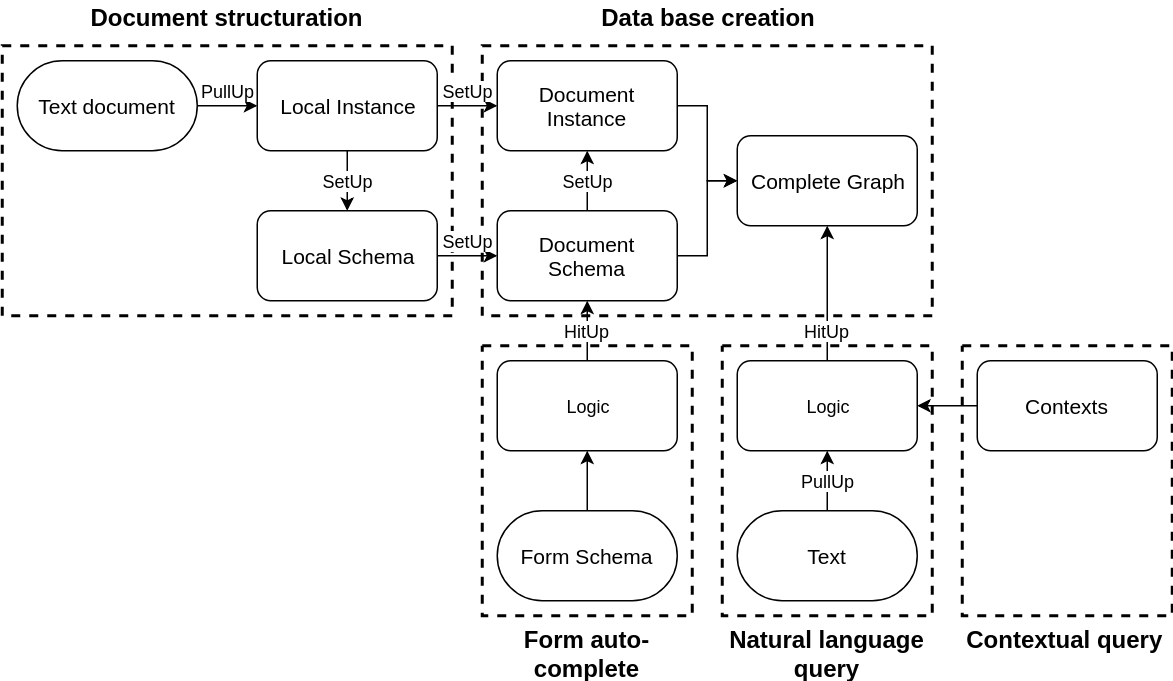
\includegraphics[width=\linewidth]{these/images/global_project.png}
    \caption{Schéma du projet}
    \label{fig:sch_projet}
\end{figure}

\paragraph{\gls{pullup}} est la partie s'occupant de l'extraction d'information.
Elle a pour objectif d'extraire les connaissances contenues dans un texte formulé en langage naturel sous forme de faits logique pouvant être utilisés pour construire notre base de données par la suite.

\paragraph{\gls{setup}} est un ensemble de travaux visant à construire dynamiquement une base de données cohérente par l'intermédiaire de grammaire de graphe \cite{chabin_using_2019}.
Ces travaux sont réalisés conjointement avec l'équipe SDS du \gls{lifo}.
Ils devraient permettre de s'assurer que la base reste cohérente sachant que l'on ne connaît pas la structure des données en entrée (car elles sont extraites depuis différents documents) et qu'on ne connaît pas le schéma de notre base (le schéma est propre aux documents présents dans la \gls{ged} et donc propre à chaque client).
Bien que le processus puisse être réalisé manuellement, cette partie du projet vise donc à automatiser la construction de la base spécifique permettant de formuler des requêtes plus adaptées aux données qu'elle contient.

\paragraph{\gls{hitup}} est une extension du formalisme présenté par \cite{chabin_context-driven_2018}.
Il vise à fournir un langage de requête permettant d'effectuer des requêtes statistiques tout en ajoutant, via des réécritures, un contexte à la requête.
Ce dernier peut être composé de contraintes d'intégrité ou de règles d'inférence utilisées pour spécifier la requête.

\section{Exemple}
\begin{quote}
    Un patient de 78 ans suivi pour cancer prostatique avec métastases ganglionnaires ayant déjà subi une résection endoscopique prostatique avec pulpectomie a été admis en urgence pour insuffisance rénale aiguë obstructive à 330 mmol/l de créatinine avec fièvre et urétérohydronéphrose bilatérale à l'échographie.
\end{quote}

\begin{align}
    CasClinique(\textit{c-2-3})  & exam(p_1, e_1, et_1, \textit{01-01-01}) \\
    hasPatient(\textit{c-2-3}, p1) & paramClinique(e_1, creatine, \textit{330mmol/L}) \\
    Patient(p_1, 78, H)  & reveal(e_1, \textit{insuffisance rénale}) \\
    hasPatho(p_1, cancer)  & exam(p_1, e_2, et_2, \textit{01-01-01}) \\
    concernsAnat(cancer, prostate) & paramClinique(e_2, temperature, t_1) \\
    Anatomy(prostate)  & reveal(e_2, fievre)  & exam(p_1, e_3, \textit{echographie}, \textit{01-01-01}) \\
    leadTo(cancer, \textit{métastases ganglionnaires})  & paramClinique(e_3, param_1, res_1) \\
    getTreatment(\textit{résection endoscopique}, prostate) & reveal(e_3, \textit{urétérohydronéphrose bilatérale}) \\
    forPatho(\textit{résection endoscopique}, cancer)
\end{align}

\begin{figure}
    \small
    \centering
    \begin{adjustbox}{varwidth=\linewidth,max height=\textheight}
        \begin{tikzpicture}[shorten >=2pt,thick,-Latex,node distance=3cm and 5cm,on grid]
            \node[labeled node] (patient) {Patient \nodepart{two} name: \emph{$p_1$}\\sex: \emph{H}\\age: \emph{78}};
            \node[labeled node, below=of patient] (exam1) {Exam \nodepart{two} name: \emph{constantes}};
            \node[labeled node, below=of exam1] (param1) {ParamClinique \nodepart{two} name: \emph{créatinine}\\value: \emph{330 mmol/l}};
            \node[labeled node, below=of param1] (sosy1) {SOSY \nodepart{two} name: \emph{insuffisance}\\~~~~~~~~~~\emph{rénale}};
            \node[labeled node, right=of exam1] (exam2) {Exam \nodepart{two} name: \emph{échographie}};
            \node[labeled node, below=of exam2] (param2) {ParamClinique \nodepart{two} name: \emph{unknown}\\ value: \emph{unknown}};
            \node[labeled node, below=of param2] (sosy2) {SOSY \nodepart{two} name: \emph{urétérohydronéphrose}\\~~~~~~~~~~\emph{bilatérale}};
            \node[labeled node, left=of param1] (param3) {ParamClinique \nodepart{two} name: \emph{temperature}\\ value: \emph{unknown}};
            \node[labeled node, below=of param3] (sosy3) {SOSY \nodepart{two} name: \emph{fièvre}};
            \node[labeled node, above=of param3] (cas) {CasClinique \nodepart{two} doc: \emph{c-2-3}};
            \node[labeled node, above=of cas] (testicule) {Anatomie \nodepart{two} name: \emph{testicule}};
            \node[labeled node, above=of patient] (traitement) {Traitement};
            \node[labeled node, above=of traitement] (traitmentType) {TraitmentType \nodepart{two} name: \emph{résection}\\~~~~~~~~~~\emph{endoscopique}};
            \node[labeled node, above=of testicule] (traitement2) {Traitement};
            \node[labeled node, above=of traitement2] (traitmentType2) {TraitmentType \nodepart{two} name: \emph{pulpectomie}};
            \node[labeled node, above=of exam2] (metastase) {Symptom \nodepart{two} name: \emph{métastases}\\~~~~~~~~~~\emph{ganglionnaires}};
            \node[labeled node, above=of metastase] (cancer) {Pathologie \nodepart{two} name: \emph{cancer}};
            \node[labeled node, above=of cancer] (prostate) {Anatomie \nodepart{two} name: \emph{prostate}};

            \path
            (cas) edge node[labeled edge, anchor=center] {hasPatient} (patient)
            (patient) edge node[labeled edge, anchor=center] {hasPatho} (cancer)
            (patient) edge node[labeled edge, anchor=center] {getTreatment} (traitement)
            (cancer) edge node[labeled edge, anchor=center] {concernsAnat} (prostate)
            (patient) edge node[labeled edge, anchor=center] {getTreatment} (traitement2)
            (cancer) edge node[labeled edge, anchor=center] {leadTo} (metastase)
            (traitement) edge node[labeled edge, anchor=center] {forPatho} (cancer)
            (traitement) edge node[labeled edge, anchor=center] {concernsAnat} (prostate)
            (traitement) edge node[labeled edge, anchor=center] {hasType} (traitmentType)
            (traitement2) edge node[labeled edge, anchor=center] {concernsAnat} (testicule)
            (traitement2) edge node[labeled edge, anchor=center] {hasType} (traitmentType2)
            (patient) edge node[labeled edge, anchor=center] {passExam} (exam1)
            (exam1) edge node[labeled edge, anchor=center] {reveal} (param1)
            (param1) edge node[labeled edge, anchor=center] {show} (sosy1)
            (patient) edge node[labeled edge, anchor=center] {passExam} (exam2)
            (exam2) edge node[labeled edge, anchor=center] {reveal} (param2)
            (param2) edge node[labeled edge, anchor=center] {show} (sosy2)
            (exam1) edge node[labeled edge, anchor=center] {reveal} (param3)
            (param3) edge node[labeled edge, anchor=center] {show} (sosy3)
            ;
        \end{tikzpicture}
    \end{adjustbox}
    \caption{Instance sous forme de graphe}
    \label{fig:runex:graph}
\end{figure}


\section{Organisation du manuscrit}

\section{Publications}


\chapter{État de l'art}
\section{Introduction}
\subfile{chapter_1/introduction}
\vfill
\pagebreak
\section{Préliminaires}
\label{sec:update:pre}
\subfile{chapter_1/preliminaires}

\section{Travaux connexes}
\label{sec:update:soa}
\subfile{chapter_1/state_of_the_art}

\subsection{SETUP : Grammaire de graphe pour la mise à jour de base RDFS}
\label{sec:update:soa:sendup}
\subfile{chapter_1/sendup_eval}

\subsection{Dépendances fonctionnelles pour les graphes}
\label{sec:update:soa:graphdeps}
\subfile{chapter_1/graph_deps}

\section{Discussion}
\label{sec:update:discussion}
\subfile{chapter_1/discussion}


\chapter{Maintien de la cohérence}
\subfile{chapter_2/state_of_the_art}

\section{SendUP}
\subfile{chapter_2/sendup_eval}


\chapter{Mise à jour incrémentale}
\section{Modélisation de la base de données sous Neo4J}
\subfile{chapter_3/graph_design}

\section{Réduction incrémentale de la redondance}
\subfile{chapter_3/core}

\section{Chase incrémentale et effet de bords}
\subfile{chapter_3/chase}

\section{Mise à jour incrémentale}
\subfile{chapter_3/update}


\chapter{Conclusion}
Nous avons examiné deux applications directes des différentes méthodes utilisées dans cette thèse dans des contextes variés.
Cela met en lumière l'efficacité de ces méthodes pour un vocabulaire contrôlé et avec peu de données d'apprentissage.
Dans le cadre d'\gls{ennov}, il est essentiel de combiner des lexiques avec des méthodes d'apprentissage plus traditionnelles.
En effet, même si deux clients peuvent manipuler les mêmes catégories d'objets dans leur base de données (telles que des personnes, des produits, etc.), les valeurs peuvent différer considérablement.
L'utilisation de lexiques permet d'éviter d'entrainer un modèle pour chaque base de données et évite également d'avoir besoin d'accéder aux données des clients, puisque les lexiques sont construits automatiquement et localement.
Notre approche montre que les lexiques constituent une ressource riche, facilement mise à jour et permettent d'obtenir une bonne qualité pour l'extraction d'entités et la classification de documents.
Nous avons également vu que le filtrage automatique de termes trop génériques fonctionne bien pour du vocabulaire spécifique.

En ce qui concerne la classification, nous avons constaté que le système proposé offre de bons résultats et surpasse les approches basées sur l'apprentissage automatique proposées lors de \gls{deft} 2021.
Contrairement aux méthodes d'apprentissage, notre approche basée sur les lexiques ne nécessite pas d'apprentissage initial (à l'exception du raffinement), ni de grands corpus d'entraînement.
De plus, elle est facilement mise à jour (il est possible d'ajouter ou de supprimer des valeurs sans nécessiter un réapprentissage du modèle) et elle est performante (la classification de \num{108} documents s'exécute en environ une minute avec notre système).
L'impact en ressources utilisées est réduit et un tel système aussi être facilement déployé sur des systèmes embarqués.

Cela met en perspective l'utilisation quasi systématique de l'apprentissage automatique, notamment des réseaux de neurones et des modèles de langue (\acrshortpl{llm}), dans l'industrie, malgré les coûts élevés et l'impact environnemental de ces solutions.
Selon \cite{strubellEnergyPolicyConsiderations2019}, l'entraînement d'un modèle de réseau de neurones profond \textquote{à l'état de l'art} pour effectuer de la traduction équivaut à l'impact de la durée de vie de cinq voitures.
De plus, les durées d'entraînement pour ces modèles peuvent varier de quelques jours à plusieurs semaines.
Il est donc important de continuer à considérer les approches symboliques, qui demeurent efficaces pour certaines tâches.

Le traitement de la négation, tel qu'abordé dans la section~\ref{sec:class:neg}, constitue une version simplifiée de la problématique.
Dans le cadre de futurs travaux, il serait envisageable de mettre en place une méthode sémantique visant à mieux identifier la portée des marqueurs de négation.
La détection de la négation peut aussi être considéré comme le problème de la détection de la portée de la contextualisation et pourrait être réalisée par une cascade de \acrshortpl{crf}.
De plus, il pourrait être intéressant d'explorer la détection de négations plus complexes, comme dans la phrase \textquote{Elle n'a présenté des nausées que durant la nuit et aucun vomissement}.
Par ailleurs, il serait également pertinent de pouvoir extraire la temporalité et la causalité au sein des textes médicaux, car ces éléments représentent des informations capitales pour la compréhension des cas cliniques.

Pour aller plus loin dans l'extraction d'information, nous avons proposé dans \cite{savaryRelationExtractionClinical2022} d'extraire un ensemble de relations médicales couramment rencontrées dans la littérature.
Cette approche repose sur un ensemble de règles appliquées sur l'arbre de dépendances et exploite le fait que la relation entre deux entités est entièrement déterminée par les types de ces entités.
Malgré les limites discutées dans la section~\ref{sec:tal:ctx:rule} pour la contextualisation des entités dans des phrases complexes, les résultats obtenus dans \cite{savaryRelationExtractionClinical2022} sont encourageants.
En effet, avec un ensemble restreint de sept règles simples, le système proposé atteint un rappel de \num{0.84}, une précision de \num{0.95} et une mesure F1 de \num{0.89}.

Les outils présentés dans ce chapitre ne constituent qu'une première étape dans le processus d'extraction d'informations.
La structuration automatique des informations, telle que présentée dans le chapitre~\ref{chp:struct}, représente une seconde étape cruciale permettant de stocker ces informations dans des bases de données.
Leur stockage facilite l'interrogation, l'exploitation et le raisonnement efficace sur ces données afin d'extraire de la connaissance.


%%%%%%%%%%%%%%%%%%

\part{Intégration de données textuelles}

\chapter{Introduction}
\section{Un peu de contexte}

\subsection{Les acteurs}
\paragraph{}
Ces travaux sont menés conjointement par le \gls{lifo} et la société \gls{ennov}.
\gls{ennov} est un éditeur de logiciels spécialisé dans le domaine médical.
Ils proposent une suite logicielle pour la gestion de contenus ainsi que l’automatisation des processus métier et des processus réglementaires.
Cela permet aux sociétés des sciences de la vie de réduire les risques réglementaires et de faciliter le respect des normes internationales.
\gls{ennov} est certifié ISO9001: 2015 pour tous ses produits et activités.
Ils offrent une meilleure capacité de prise de décision, une automatisation des tâches répétitives et une visibilité accrue dans toute l'organisation.
\gls{ennov} est hautement évolutif, mais facilement implémenté, conçu pour une utilisation minimale de l'infrastructure informatique, des coûts ou des ressources.

\gls{ennov} est reconnu par \gls{gartner} comme un fournisseur pertinent pour le \gls{rim} / \gls{idmp} ainsi qu'un fournisseur mondial de technologies logicielles pour les sociétés des sciences de la vie.
La suite logicielle d'\gls{ennov} comprend des fonctions de gestion de processus et de contenu pour la gestion de la qualité, les affaires réglementaires, les études cliniques et la pharmacovigilance.

\gls{ennov} a pour objectif de concevoir des solutions logicielles interconnectées qui s'intègrent aux flux de travail.
L'ensemble de la suite logicielle est basée sur une \gls{ged} qui est chargée de la gestion du cycle de vie des documents.
Ces travaux vont permettre une meilleure utilisation des données disponibles afin d'obtenir des gains de productivité.

\paragraph{}
Le \gls{lifo} est un laboratoire de l'université d'Orléans et de l'\gls{insa} Centre-Val de Loire.
Les recherches qui sont menées au \gls{lifo} vont de l'algorithmique au traitement des langues naturelles, de l'apprentissage au parallélisme massif, de la vérification et la certification à la sécurité des systèmes, du Big Data aux systèmes embarqués.

Le \gls{lifo} est composé de cinq équipes :
\begin{description}
 \item[CA] Contraintes et Apprentissage
 \item[GAMoC] Graphes, Algorithmes et Modèles de Calcul
 \item[LMV] Logique, Modélisation et Vérification
 \item[Pamda] Parallélisme, Calcul distribué et Base de donnés
 \item[SDS] Sécurité des Données et des Systèmes
\end{description}

\section{Le projet}
L'extraction des informations contenues dans un texte, sa structuration, sa classification et son étude statistiques représente un challenge, mais aussi une grande plus-value concernant le domaine de la pharmacovigilance.
Ce dernier consiste à suivre les cas d'effet secondaire liée à différents médicaments.
Il est important de connaître l'historique de chaque patient ainsi que le déroulement précis des évènements pour déduire la cause des effets secondaires.
Ces informations sont recueillies par des centres d'appels qui ont pour mission de fournir un document standardisé auprès des autorités de santé.
Comme dit précédemment les informations contenues dans ce document, pourtant essentiel pour déduire les causes, ne sont pas accessibles par un traitement automatique.
Il est donc nécessaire de fournir manuellement toutes ces informations.
Cela représente une grande quantité de données et donc un temps de travail et un coût plus important sans oublier que c'est un processus à fort risque d'erreur.

La pharmacovigilance est donc l'emploi idéal de telle recherche, car il est important de pouvoir extraire cette information et de faciliter, par la suite, leur compréhension et leur analyse avec des requêtes plus évoluées permettant à l'avenir de concevoir un système-expert.
Ces travaux ont pour vocation d'être intégré à la suite \gls{ennov} que ce soit dans la \gls{ged} ou dans la partie logicielle traitant de la pharmacovigilance.

\paragraph{}
L'interrogation du contenu des documents implique que ces données soient facilement accessibles et de façon structurée, ce qui n'est pas le cas dans un document textuel.
Le projet se découpe donc en deux axes, dans un premier temps, il s'agit d'extraire l'information, la structurer et la stocker.
Dans un second temps, il faut proposer un formalisme d'interrogation basé sur le contexte permettant des analyses statistiques dans une base de données et permettre la traduction d'une requête en langage naturel vers ce formalisme.

\paragraph{}
Pour construire une base de connaissance cohérente et structurée, il faut commencer par extraire les données contenues dans les documents.
Ce processus se nomme : \gls{ie} (\cite{grishman_information_1997,cowie_information_2000}) et représente un axe de recherche du \gls{tal}.
Certains travaux portent déjà sur l'extraction d'information notamment dans un domaine médical \cite{polepalli_ramesh_automatically_2014}, cependant, ils ne permettent pas d'obtenir une structure cohérente pour ces données et il est donc peu envisageable de tenter d'y retrouver de l'information sans un traitement préalable.
N'existant pas de solution nous permettant d'obtenir le résultat souhaité, ceci constitue un des axes de recherche du projet.

Le second axe de recherche porte sur la formulation de requête statistique enrichie d'un contexte \cite{chabin_context-driven_2018}.
Le contexte est une suite de règles permettant de préciser la requête initiale.
Dans le cadre du projet, ces travaux rendront personnalisé les requêtes utilisateurs, car chacun se verra attribuer un contexte qui lui est propre.
Le contexte servira aussi pour l'extraction d'information.

\paragraph{}
Le projet est donc découpé en plusieurs parties regroupées sous différents modules.
La figure~\ref{fig:sch_projet} présente les cinq modules du projet ainsi que les différentes parties en précisant les travaux qui les lient.

\begin{figure}[htb]
    \centering
    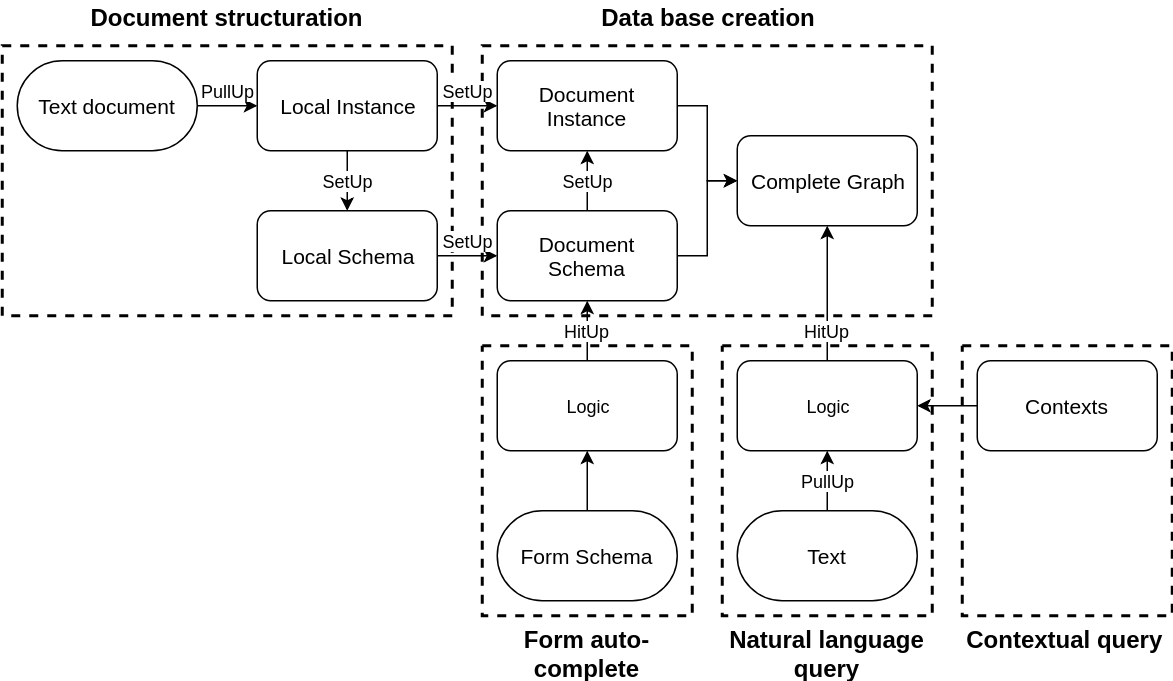
\includegraphics[width=\linewidth]{these/images/global_project.png}
    \caption{Schéma du projet}
    \label{fig:sch_projet}
\end{figure}

\paragraph{\gls{pullup}} est la partie s'occupant de l'extraction d'information.
Elle a pour objectif d'extraire les connaissances contenues dans un texte formulé en langage naturel sous forme de faits logique pouvant être utilisés pour construire notre base de données par la suite.

\paragraph{\gls{setup}} est un ensemble de travaux visant à construire dynamiquement une base de données cohérente par l'intermédiaire de grammaire de graphe \cite{chabin_using_2019}.
Ces travaux sont réalisés conjointement avec l'équipe SDS du \gls{lifo}.
Ils devraient permettre de s'assurer que la base reste cohérente sachant que l'on ne connaît pas la structure des données en entrée (car elles sont extraites depuis différents documents) et qu'on ne connaît pas le schéma de notre base (le schéma est propre aux documents présents dans la \gls{ged} et donc propre à chaque client).
Bien que le processus puisse être réalisé manuellement, cette partie du projet vise donc à automatiser la construction de la base spécifique permettant de formuler des requêtes plus adaptées aux données qu'elle contient.

\paragraph{\gls{hitup}} est une extension du formalisme présenté par \cite{chabin_context-driven_2018}.
Il vise à fournir un langage de requête permettant d'effectuer des requêtes statistiques tout en ajoutant, via des réécritures, un contexte à la requête.
Ce dernier peut être composé de contraintes d'intégrité ou de règles d'inférence utilisées pour spécifier la requête.

\section{Exemple}
\begin{quote}
    Un patient de 78 ans suivi pour cancer prostatique avec métastases ganglionnaires ayant déjà subi une résection endoscopique prostatique avec pulpectomie a été admis en urgence pour insuffisance rénale aiguë obstructive à 330 mmol/l de créatinine avec fièvre et urétérohydronéphrose bilatérale à l'échographie.
\end{quote}

\begin{align}
    CasClinique(\textit{c-2-3})  & exam(p_1, e_1, et_1, \textit{01-01-01}) \\
    hasPatient(\textit{c-2-3}, p1) & paramClinique(e_1, creatine, \textit{330mmol/L}) \\
    Patient(p_1, 78, H)  & reveal(e_1, \textit{insuffisance rénale}) \\
    hasPatho(p_1, cancer)  & exam(p_1, e_2, et_2, \textit{01-01-01}) \\
    concernsAnat(cancer, prostate) & paramClinique(e_2, temperature, t_1) \\
    Anatomy(prostate)  & reveal(e_2, fievre)  & exam(p_1, e_3, \textit{echographie}, \textit{01-01-01}) \\
    leadTo(cancer, \textit{métastases ganglionnaires})  & paramClinique(e_3, param_1, res_1) \\
    getTreatment(\textit{résection endoscopique}, prostate) & reveal(e_3, \textit{urétérohydronéphrose bilatérale}) \\
    forPatho(\textit{résection endoscopique}, cancer)
\end{align}

\begin{figure}
    \small
    \centering
    \begin{adjustbox}{varwidth=\linewidth,max height=\textheight}
        \begin{tikzpicture}[shorten >=2pt,thick,-Latex,node distance=3cm and 5cm,on grid]
            \node[labeled node] (patient) {Patient \nodepart{two} name: \emph{$p_1$}\\sex: \emph{H}\\age: \emph{78}};
            \node[labeled node, below=of patient] (exam1) {Exam \nodepart{two} name: \emph{constantes}};
            \node[labeled node, below=of exam1] (param1) {ParamClinique \nodepart{two} name: \emph{créatinine}\\value: \emph{330 mmol/l}};
            \node[labeled node, below=of param1] (sosy1) {SOSY \nodepart{two} name: \emph{insuffisance}\\~~~~~~~~~~\emph{rénale}};
            \node[labeled node, right=of exam1] (exam2) {Exam \nodepart{two} name: \emph{échographie}};
            \node[labeled node, below=of exam2] (param2) {ParamClinique \nodepart{two} name: \emph{unknown}\\ value: \emph{unknown}};
            \node[labeled node, below=of param2] (sosy2) {SOSY \nodepart{two} name: \emph{urétérohydronéphrose}\\~~~~~~~~~~\emph{bilatérale}};
            \node[labeled node, left=of param1] (param3) {ParamClinique \nodepart{two} name: \emph{temperature}\\ value: \emph{unknown}};
            \node[labeled node, below=of param3] (sosy3) {SOSY \nodepart{two} name: \emph{fièvre}};
            \node[labeled node, above=of param3] (cas) {CasClinique \nodepart{two} doc: \emph{c-2-3}};
            \node[labeled node, above=of cas] (testicule) {Anatomie \nodepart{two} name: \emph{testicule}};
            \node[labeled node, above=of patient] (traitement) {Traitement};
            \node[labeled node, above=of traitement] (traitmentType) {TraitmentType \nodepart{two} name: \emph{résection}\\~~~~~~~~~~\emph{endoscopique}};
            \node[labeled node, above=of testicule] (traitement2) {Traitement};
            \node[labeled node, above=of traitement2] (traitmentType2) {TraitmentType \nodepart{two} name: \emph{pulpectomie}};
            \node[labeled node, above=of exam2] (metastase) {Symptom \nodepart{two} name: \emph{métastases}\\~~~~~~~~~~\emph{ganglionnaires}};
            \node[labeled node, above=of metastase] (cancer) {Pathologie \nodepart{two} name: \emph{cancer}};
            \node[labeled node, above=of cancer] (prostate) {Anatomie \nodepart{two} name: \emph{prostate}};

            \path
            (cas) edge node[labeled edge, anchor=center] {hasPatient} (patient)
            (patient) edge node[labeled edge, anchor=center] {hasPatho} (cancer)
            (patient) edge node[labeled edge, anchor=center] {getTreatment} (traitement)
            (cancer) edge node[labeled edge, anchor=center] {concernsAnat} (prostate)
            (patient) edge node[labeled edge, anchor=center] {getTreatment} (traitement2)
            (cancer) edge node[labeled edge, anchor=center] {leadTo} (metastase)
            (traitement) edge node[labeled edge, anchor=center] {forPatho} (cancer)
            (traitement) edge node[labeled edge, anchor=center] {concernsAnat} (prostate)
            (traitement) edge node[labeled edge, anchor=center] {hasType} (traitmentType)
            (traitement2) edge node[labeled edge, anchor=center] {concernsAnat} (testicule)
            (traitement2) edge node[labeled edge, anchor=center] {hasType} (traitmentType2)
            (patient) edge node[labeled edge, anchor=center] {passExam} (exam1)
            (exam1) edge node[labeled edge, anchor=center] {reveal} (param1)
            (param1) edge node[labeled edge, anchor=center] {show} (sosy1)
            (patient) edge node[labeled edge, anchor=center] {passExam} (exam2)
            (exam2) edge node[labeled edge, anchor=center] {reveal} (param2)
            (param2) edge node[labeled edge, anchor=center] {show} (sosy2)
            (exam1) edge node[labeled edge, anchor=center] {reveal} (param3)
            (param3) edge node[labeled edge, anchor=center] {show} (sosy3)
            ;
        \end{tikzpicture}
    \end{adjustbox}
    \caption{Instance sous forme de graphe}
    \label{fig:runex:graph}
\end{figure}


\section{Organisation du manuscrit}

\section{Publications}


\chapter{Structuration d'informations}
\section{Introduction}
\subfile{chapter_1/introduction}

\section{Préliminaires}
\label{sec:struct:pre}
\subfile{chapter_1/preliminaires}

\section{Une grammaire comme schéma}
\label{sec:struct:meta}
\subfile{chapter_1/schema}

\section{Structuration automatique}
\label{sec:struct:steps}
\subfile{chapter_1/steps}

\section{Proposition d'implémentation}
\label{sec:struct:implem}
\subfile{chapter_1/algo}

\section{Évaluation préliminaire}
\label{sec:struct:eval}
\subfile{chapter_1/evaluation}

\section{Conclusion}
\label{sec:struct:conclusion}
\subfile{chapter_1/conclusion}


\chapter{Extraction d'informations}
\section{Introduction}
\subfile{chapter_2/introduction}

\section{Analyse syntaxique}
\subfile{chapter_2/syntax}

\section{Extraction par lexiques}
\label{sec:ie:lexicon}
\subfile{chapter_2/lexicon}

\section{Entités ambiguës et contextualisation}
\subfile{chapter_2/entity}

\section{Classification de cas cliniques}
\subfile{chapter_2/Classification}

\section{Interrogation de base de données en langue naturelle}
\subfile{chapter_2/nl-queries}

\section{Conclusion}
\subfile{chapter_2/conclusion}


\chapter{Conclusion}
Nous avons examiné deux applications directes des différentes méthodes utilisées dans cette thèse dans des contextes variés.
Cela met en lumière l'efficacité de ces méthodes pour un vocabulaire contrôlé et avec peu de données d'apprentissage.
Dans le cadre d'\gls{ennov}, il est essentiel de combiner des lexiques avec des méthodes d'apprentissage plus traditionnelles.
En effet, même si deux clients peuvent manipuler les mêmes catégories d'objets dans leur base de données (telles que des personnes, des produits, etc.), les valeurs peuvent différer considérablement.
L'utilisation de lexiques permet d'éviter d'entrainer un modèle pour chaque base de données et évite également d'avoir besoin d'accéder aux données des clients, puisque les lexiques sont construits automatiquement et localement.
Notre approche montre que les lexiques constituent une ressource riche, facilement mise à jour et permettent d'obtenir une bonne qualité pour l'extraction d'entités et la classification de documents.
Nous avons également vu que le filtrage automatique de termes trop génériques fonctionne bien pour du vocabulaire spécifique.

En ce qui concerne la classification, nous avons constaté que le système proposé offre de bons résultats et surpasse les approches basées sur l'apprentissage automatique proposées lors de \gls{deft} 2021.
Contrairement aux méthodes d'apprentissage, notre approche basée sur les lexiques ne nécessite pas d'apprentissage initial (à l'exception du raffinement), ni de grands corpus d'entraînement.
De plus, elle est facilement mise à jour (il est possible d'ajouter ou de supprimer des valeurs sans nécessiter un réapprentissage du modèle) et elle est performante (la classification de \num{108} documents s'exécute en environ une minute avec notre système).
L'impact en ressources utilisées est réduit et un tel système aussi être facilement déployé sur des systèmes embarqués.

Cela met en perspective l'utilisation quasi systématique de l'apprentissage automatique, notamment des réseaux de neurones et des modèles de langue (\acrshortpl{llm}), dans l'industrie, malgré les coûts élevés et l'impact environnemental de ces solutions.
Selon \cite{strubellEnergyPolicyConsiderations2019}, l'entraînement d'un modèle de réseau de neurones profond \textquote{à l'état de l'art} pour effectuer de la traduction équivaut à l'impact de la durée de vie de cinq voitures.
De plus, les durées d'entraînement pour ces modèles peuvent varier de quelques jours à plusieurs semaines.
Il est donc important de continuer à considérer les approches symboliques, qui demeurent efficaces pour certaines tâches.

Le traitement de la négation, tel qu'abordé dans la section~\ref{sec:class:neg}, constitue une version simplifiée de la problématique.
Dans le cadre de futurs travaux, il serait envisageable de mettre en place une méthode sémantique visant à mieux identifier la portée des marqueurs de négation.
La détection de la négation peut aussi être considéré comme le problème de la détection de la portée de la contextualisation et pourrait être réalisée par une cascade de \acrshortpl{crf}.
De plus, il pourrait être intéressant d'explorer la détection de négations plus complexes, comme dans la phrase \textquote{Elle n'a présenté des nausées que durant la nuit et aucun vomissement}.
Par ailleurs, il serait également pertinent de pouvoir extraire la temporalité et la causalité au sein des textes médicaux, car ces éléments représentent des informations capitales pour la compréhension des cas cliniques.

Pour aller plus loin dans l'extraction d'information, nous avons proposé dans \cite{savaryRelationExtractionClinical2022} d'extraire un ensemble de relations médicales couramment rencontrées dans la littérature.
Cette approche repose sur un ensemble de règles appliquées sur l'arbre de dépendances et exploite le fait que la relation entre deux entités est entièrement déterminée par les types de ces entités.
Malgré les limites discutées dans la section~\ref{sec:tal:ctx:rule} pour la contextualisation des entités dans des phrases complexes, les résultats obtenus dans \cite{savaryRelationExtractionClinical2022} sont encourageants.
En effet, avec un ensemble restreint de sept règles simples, le système proposé atteint un rappel de \num{0.84}, une précision de \num{0.95} et une mesure F1 de \num{0.89}.

Les outils présentés dans ce chapitre ne constituent qu'une première étape dans le processus d'extraction d'informations.
La structuration automatique des informations, telle que présentée dans le chapitre~\ref{chp:struct}, représente une seconde étape cruciale permettant de stocker ces informations dans des bases de données.
Leur stockage facilite l'interrogation, l'exploitation et le raisonnement efficace sur ces données afin d'extraire de la connaissance.


%%%%%%%%%%%%%%%%%%

\part{Conclusion et perspectives}
\section{Contributions}

Nous avons présenté dans ce manuscrit un ensemble de travaux pour la construction automatique de bases de données pour le domaine médical.
En particulier, nos recherches se focalisent sur les bases de données graphes pouvant contenir des données incomplètes et s'articulent autour de deux axes principaux :
\begin{itemize}
    \item La maintenance et le maintien de la cohérence d'une base de données incomplète par rapport à un ensemble de règles définies.

    \item L'extraction et la structuration automatique d'informations à partir de textes en vue de leur intégration dans une base de données.
\end{itemize}

Dans la suite de cette section, nous détaillerons les contributions majeures réalisées sur ces deux axes.

\subsection{\nameref*{part:update}}

Maintenir une base de données cohérente est essentiel pour faciliter l'analyse des données.
Cette tâche devient particulièrement complexe lorsque la base de données peut contenir des données incomplètes, matérialisées par des valeurs nulles liées.
Dans la première partie de ce manuscrit, nous avons examiné une politique de maintenance qui accorde la priorité aux mises à jour.
Concrètement, au lieu de rejeter des mises à jour susceptibles de rendre les données incohérentes, nous cherchons à effectuer les modifications nécessaires pour que ces mises à jour soient applicables.
À cette fin, nous avons proposé une extension des travaux de \cite{chabinConsistentUpdatingDatabases2020} basée sur la sémantique de \cite{reiterSoundSometimesComplete1986} et qui ne limite pas le pouvoir d'expressivité des contraintes.
Contrairement à l'approche en mémoire présentée dans \cite{chabinConsistentUpdatingDatabases2020}, nos travaux se concentrent sur la maintenance en relation avec un \gls{sgbd}.

Notre extension comporte les contributions suivantes :
\begin{itemize}
    \item Une modélisation d'un graphe attribué visant à optimiser les différentes opérations requises pour assurer la cohérence de la base de données, en particulier pour la recherche des atomes liés, une opération coûteuse dans une modélisation classique dans une base de données relationnelle.
    
    \item Une procédure de mise à jour incrémentale, en mode connecté, reposant sur un ensemble de requêtes.
\end{itemize}

L'évaluation présentée dans la section~\ref{sec:update:evaluation} (page~\pageref{sec:update:evaluation}) met en lumière l'évolution significative des performances de notre approche incrémentale par rapport à l'approche complète proposée dans \cite{chabinConsistentUpdatingDatabases2020}, malgré l'interaction avec un \gls{sgbd}.
Cette étude des performances souligne également les qualités de notre modèle de graphe, qui permet de réduire de manière significative le coût de la recherche des atomes liés en construisant un graphe similaire à \acrshort{rdf}, où les individus sont représentés par des nœuds.
Toutefois, elle met également en évidence les limitations du modèle de graphe, où les performances des requêtes dépendent fortement de la modélisation.
Dans notre cas, la fragmentation des données en un grand nombre de nœuds et de relations rend la recherche d'homomorphismes difficile.

\subsection{\nameref*{part:texts}}

Ce second axe de recherche concerne l'exploitation des informations contenues dans les textes.
L'approche proposée repose sur des techniques d'extraction d'information, en particulier l'extraction d'entités.
Le cœur de ces travaux réside dans la structuration automatique des informations.
Dans ce contexte, ce manuscrit propose :
\begin{itemize}
    \item Un méta-modèle permettant d'organiser les informations de manière cohérente ;

    \item Une méta-grammaire capable de reconnaître l'ensemble des schémas valides du méta-modèle ;

    \item Une procédure itérative de structuration de l'information ;

    \item Une preuve de concept avec l'implémentation de la procédure, avec pour stratégie la minimisation de la grammaire cible.
\end{itemize}

Une évaluation préliminaire a démontré que la procédure proposée répond à la problématique et produit des résultats prometteur tant pour la structuration que pour l'intégration de données.
L'évaluation souligne également l'importance de cette étape dans la construction automatique d'une base de données à partir de données textuelles.

\paragraph{}
Dans un second temps, nous proposons différentes techniques pour l'extraction d'entités permettant de répondre aux problématiques d'accès restreint aux données, d'efficacité et d'explicabilité.
En particulier, nous proposons une approche itérative hybride reposant sur :
\begin{itemize}
    \item Une représentation multi-valuée des entités nommées, permettant de prendre en compte l'ambiguïté et l'incertitude ;
    
    \item L'utilisation de lexiques par la construction d'un \gls{fst} pour l'annotation efficace d'entités nommées ;
    
    \item La notion de contextualisation et de spécification basée sur des marqueurs, avec une approche basée sur des règles ainsi qu'une approche reposant sur une cascade de \glspl{crf}.
\end{itemize}

Nous avons également présenté deux cas d'application concrets reposant sur cette approche, l'un pour la classification de documents et l'autre pour la construction de \gls{nli} permettant l'interrogation et l'analyse de données.
Ces deux cas d'application ont permis de démontrer les performances de notre approche en obtenant des résultats satisfaisants sans recourir à un apprentissage automatique nécessitant de vastes corpus d'entraînement.
Cette approche permet ainsi de travailler efficacement avec des données sensibles ou difficilement accessibles.
Ces deux cas d'usage témoignent également de la flexibilité et de la simplicité d'adaptation du processus itératif d'extraction.

\section{Perspectives}

Les travaux présentés dans cette thèse offrent des résultats importants et ouvrent de nombreuses perspectives pour la suite.
En particulier, nous nous intéressons à trois d'entre elles que nous souhaitons développer davantage.

\subsection{Maintien de la cohérence de graphes attribués}

Dans le chapitre~\ref{chp:update:algos}, nous avons présenté un modèle de graphe attribué conçu pour répondre à la problématique de la mise à jour cohérente.
Cette représentation de la base de données vise à optimiser les interactions nécessaires au maintien de la cohérence, telles que la recherche des nœuds liés et la recherche d'homomorphismes pour le calcul du cœur.
Cette approche repose sur un modèle qui ne correspond pas nécessairement à une représentation intuitive des données, ce qui rend l'interrogation du graphe difficile, contrairement à l'approche proposée avec le modèle relationnel (voir la section~\ref{sec:update:evaluation:mysql}, page~\pageref{sec:update:evaluation:mysql}).
À l'usage, il est envisageable qu'une autre représentation des données sous forme de graphe soit utilisée pour l'interrogation par un utilisateur.

Pour répondre à cette problématique, nous envisageons d'explorer et de comparer deux approches :
\begin{enumerate}
    \item Les deux graphes existent simultanément et notre modélisation du graphe est considérée comme un index utilisé pour le maintien de la cohérence.
    Cette approche implique un coût de maintenance supplémentaire pour maintenir les deux représentations à jour.
    Elle s'inscrit dans la perspective d'utiliser des bases de données hybrides \cite{hassanGRFusionGraphsFirstClass2018} permettant d'exploiter efficacement le modèle relationnel et le modèle de graphe attribué de manière simultanée.

    \item Seule notre représentation est utilisée pour la sauvegarde en base, mais l'ensemble des requêtes émises lors de l'interrogation est automatiquement traduit vers notre modélisation.
    Cette approche pourrait simplifier la maintenance, mais elle pourrait également entraîner des coûts supplémentaires lors de la traduction des requêtes, surtout si elles sont complexes \cite{sujanskyHeterogeneousDatabaseIntegration2001,asfand-e-yarSemanticIntegrationHeterogeneous2020}.
\end{enumerate}

Dans la section~\ref{sec:update:evaluation} (page~\pageref{sec:update:evaluation}), nous avons examiné les coûts engendrés par notre modélisation pour la recherche d'homomorphismes.
Une perspective de ces travaux consiste à proposer l'application de notre politique de mise à jour sur un graphe attribué plus intuitif pour améliorer la recherche des homomorphismes.
Bien que cette approche ait été envisagée dans nos travaux, elle présente les défis suivants :
\begin{enumerate}
    \item Dans un graphe quelconque, l'incomplétude peut se situer au niveau des propriétés d'un nœud ou d'une relation, mais peut également concerner les nœuds ou les relations eux-mêmes.
    Cette approche complexifie grandement la recherche des valeurs nulles et la détection des ensembles liés.

    \item Dans notre approche, nous proposons une vision \acrshort{rdf} où les individus sont les termes de nos faits logiques.
    En revanche, dans le cadre des graphes de propriété, les individus sont des nœuds, et il est donc nécessaire de définir quand deux nœuds sont équivalents pour le calcul du \gls{core}.
    Contrairement au modèle relationnel, les graphes n'ont pas de notion de dépendances fonctionnelles ni de clés.
    Bien que des travaux tentent de répondre à cette question, comme nous l'avons vu avec les \gls{gfd} \cite{fanDependenciesGraphs2019}, cette question n'est pas encore résolue.
\end{enumerate}

\subsection{Uniformisation de données pour l'application de processus}

Dans le chapitre~\ref{chp:struct} (section~\ref{sec:struct:implem:integration}, page~\pageref{sec:struct:implem:integration}), nous avons examiné comment notre approche de structuration automatique de l'information pourrait être appliquée à l'intégration de données.
En particulier, on s'intéresse à développer l'idée d'unification des données.
En effet, on remarque de plus en plus le besoin de construire des méta-modèles afin de standardiser la représentation des données et de les rendre interopérables, facilitant ainsi leur intégration et leur utilisation cohérente à travers différentes applications et systèmes.

Malgré l'existence de modèles unifiés comme les graphes \gls{rdf} et l'implémentation de l'Open Linked Data, leur adoption reste limitée.
De plus, les ontologies mises en place présentent souvent des chevauchements et les liens d'équivalence ne sont pas toujours spécifiés, ce qui requiert une vigilance accrue pour garantir une interopérabilité optimale entre les différentes sources de données \cite{rulaDataQualityIssues2016}.
Par ailleurs, un grand nombre de données proviennent généralement de divers outils utilisant des formats variés, certains étant plus structurés que d'autres.
Les bases de données sont régulièrement fragmentées avec des schémas variés, souvent pour des raisons historiques.
Il est courant que chaque service au sein d'une même entreprise enregistre ses données de manière indépendante et non uniforme afin de répondre à des besoins spécifiques.
Cette diversité de formats complique l'interrogation, l'analyse et le traitement des données.

L'adoption d'une approche uniforme pour la gestion de ces données offre des avantages significatifs dans des domaines tels que le journalisme de données en facilitant la corrélation des données provenant de différentes sources et services.
En s'appuyant sur les travaux présentés dans le chapitre~\ref{chp:struct}, notamment le méta-modèle proposé, une perspective de recherche de chercher à utiliser ce modèle pour pouvoir agréger de manière dynamique et automatique un ensemble de ressources, ainsi que l'ensemble des entrées et sorties des différents processus en place.
Cette approche permettrait de rendre un processus appliqué à des données d'une ressource également applicable aux données d'autres ressources.
Elle pourrait également faciliter l'enchaînement de divers processus et leur application sur l'ensemble des ressources disponibles de manière simultanée.

Contrairement à l'approche proposée dans le chapitre~\ref{chp:struct}, le méta-modèle servirait de représentation intermédiaire de l'ensemble des ressources.
Le défi de cette approche réside dans la capacité à identifier les correspondances entre les différentes ressources.
Une approche envisagée serait d'utiliser des mécanismes similaires à ceux présentés dans la structuration automatique pour l'identification des regroupements équivalents.
La différence majeure est que l'on ne cherche pas à construire une base unifiée, mais à identifier les transformations nécessaires pour convertir dynamiquement une ressource vers un autre format.
Plutôt que de reconstruire l'ensemble des ressources, l'idée est de fournir une couche supplémentaire d'interopérabilité, permettant ainsi une intégration dynamique et une utilisation cohérente des données provenant de différentes sources et formats.

\subsection{Base de données floues}

Dans le chapitre~\ref{chp:struct}, nous avons examiné la structuration automatique d'informations basée sur l'extraction d'entités nommées, mais qui ne repose pas sur les valeurs spécifiques associées à ces entités.
Dans le chapitre~\ref{chp:tal}, nous avons proposé une représentation multi-valuée des entités nommées pour capturer l'ambiguïté inhérente aux textes.
Une partie de cette ambiguïté peut être résolue par le contexte : par exemple, pour le mot \textquote{Paris}, qui peut faire référence à une personne ou à la ville, si la valeur est détectée comme une adresse, alors la valeur associée à la personne peut être supprimée.
Cependant, toutes les ambiguïtés ne peuvent pas être résolues de cette manière et l'insertion d'informations structurées dans une base de données implique nécessairement la résolution préalable de ces ambiguïtés.

Une perspective envisagée consiste à enregistrer les données sans résoudre leur ambiguïté, en s'appuyant sur les principes de la logique floue.
Dans cette approche, chaque valeur serait associée à une valeur de vérité comprise entre $0$ et $1$.
La valeur de vérité n'est pas nécessairement déterminée par le nombre de valeurs ambiguës, mais pourrait également refléter un certain niveau de confiance dans les données.
L'idée sous-jacente est que l'ambiguïté pourrait être résolue progressivement au fil des mises à jour : en étant contraintes par un ensemble de règles, ces dernières pourraient contribuer à clarifier l'ambiguïté.
De même, l'ambiguïté pourrait être résolue au moment de l'interrogation en croisant des résultats.
Cette valeur de vérité pourrait ensuite être utilisée pour filtrer ou organiser les résultats.

\begin{example}
    Par exemple, supposons qu'un événement ait pour adresse \emph{Paris, France} et \emph{Orléans, France}.
    Interroger la base pour obtenir l'adresse exacte pourrait renvoyer deux solutions possibles (\emph{Paris, France} et \emph{Orléans, France}), chacune avec une valeur de vérité de $0.5$.
    En revanche, si l'utilisateur demande uniquement le pays, la réponse peut être unique (\emph{France}) avec une valeur de vérité de $1$ (\SI{100}{\percent} des entrées dans la base ont la valeur \emph{France}).

    L'introduction de contraintes supplémentaires lors de la requête, telles que la ville, pourrait conduire à une réponse unique, mais la valeur de vérité est plus incertaine : elle pourrait être de $0.5$ si l'on prend en compte l'ensemble de la base de données ou de $1$ si l'on ne considère que l'ensemble des résultats de la requête.
    Cette deuxième approche est justifiable si l'on suppose que les deux réponses sont vraies, mais pas simultanément.
    Ainsi, demander l'adresse en précisant la ville reviendrait à préciser le contexte d'interrogation.
    Ce dernier point révèle l'une des difficultés de la tâche, à savoir le calcul de cette valeur de vérité et pourrait nécessiter l'ajout de la notion de contexte au moment de l'interrogation.
\end{example}

Cette idée présente des similitudes avec les solutions proposées dans le modèle relationnel pour la gestion des données temporelles \cite{kulkarniTemporalFeaturesSQL2012}.
Un parallèle peut également être établi avec les travaux sur les bases de données contextuelles \cite{stavrakasMultidimensionalSemistructuredData2002,stavrakasMultidimensionalSemistructuredData2003}.
Ces travaux s'attardent sur la représentation de données contextuelles en introduisant un modèle multidimensionnel qui se réduit à un modèle conventionnel pour un contexte donné.
La mise en place de bases de données floues pourrait également représenter un cas d'application des moteurs de recommandation, où la valeur de vérité serait propre à chaque utilisateur et correspondrait au score de recommandation.
Cette proposition soulève plusieurs questions : Comment rendre l'interrogation de données efficace dans ce contexte ? Comment calculer de manière cohérente cette valeur de vérité lors de l'interrogation, en particulier lors de l'agrégation ? Et comment garantir la cohérence de la base de données avec un ensemble de règles dans ce contexte ?


%%%%%%%%%%%%%%%%%%%%%%%%%%%%%%%%%%%%%%%%%%%%%%%%%%%%%%%%%%%%%%%%%%%%%
%Fin de la thèse
%\clearpage         % verso
\cleardoublepage    % recto-verso
%%%%%%%%%%%%%%%%%%%%%%%%%%%%%%%%%%%%%%%%%%%%%%%%%%%%%%%%%%%%%%%%%%%%%
% Appendices 
\appendix
\chapter{Méthode de calcul et preuves pour la recherche de l'homomorphisme le plus spécifique}
\label{appendice:most-specific}
\subfile{appendices/most_specific}

\chapter{Description des jeux de données (mise à jour cohérente)}
\label{appendice:datasets}
\subfile{appendices/datasets}

% \chapter{Plateforme EnnovAI}
% \subfile{appendices/eaip}

\clearpage
%%%%%%%%%%%%%%%%%%%%%%%%%%%%%%%%%%%%%%%%%%%%%%%%%%%%%%%%%%%%%%%%%%%%%
%\nocite{*}         % Pour inclure toutes les references (y compris celles qui ne sont pas citees)
\addcontentsline{toc}{part}{Bibliographie}
\bibliographystyle{plain}
\bibliography{these/biblio}
%%%%%%%%%%%%%%%%%%%%%%%%%%%%%%%%%%%%%%%%%%%%%%%%%%%%%%%%%%%%%%%%%%%%%
\printindex
